\documentclass[a4paper,11pt]{article}
\usepackage{filecontents}

\usepackage[utf8]{inputenc}
\usepackage[english]{babel}
\usepackage{graphicx, array, blindtext}
\usepackage[colorinlistoftodos]{todonotes}
\DeclareUnicodeCharacter{2212}{-}
\usepackage [a4 paper , hmargin = 1.2 in , bottom = 1.5 in] {geometry}
\usepackage [parfill] {parskip}

\usepackage{enumitem}
\usepackage{amsmath}
\usepackage{amsthm}

\usepackage{nameref}
\usepackage{amssymb}
\usepackage [linesnumbered, ruled, vlined] {algorithm2e}
\usepackage{listings}
\usepackage{xcolor}
\usepackage{floatrow}
\usepackage{siunitx}


\usepackage{cancel}
\usepackage{fancyhdr}
\usepackage{graphicx}
\usepackage{verbatim}
\usepackage[document]{ragged2e}

\renewcommand{\footrulewidth}{0.4pt}
\newtheorem{definition}{Definition}
\numberwithin{definition}{section}
\newtheorem{mytheorem}{Theorem}
\numberwithin{mytheorem}{subsection}
\newcommand{\notimplies}{\;\not\!\!\!\longrightarrow}  
\newcommand\norm[1]{\left\lVert#1\right\rVert}
\pagestyle{fancy}
\fancyhf{}
\rhead{CS754 Assignment 1}
\lhead{200050013-200050130}
\fancyfoot[C]{Page \thepage}
\usepackage{subcaption}
\usepackage{listings}


\usepackage{hyperref}
\urlstyle{same}
\hypersetup{pdftitle={main.pdf},
    colorlinks=false,
    linkbordercolor=red
}
\usepackage{array}
\usepackage{listings,chngcntr}

\begin{document}
\centering{

\title{\fontsize{150}{60}{CS754 Assignment 1 Report}}

\author{
Arpon Basu \\ Shashwat Garg }
}

% Replace photos after seed
% Align equations
% Explain each other



\date{Spring 2022}
\maketitle

\justifying
\tableofcontents

\newpage
\justifying
\section*{Introduction}

Welcome  to our report on CS754 Assignment 1. We have tried to make this report comprehensive and self-contained. We hope reading this would give you a proper flowing description of our work, methods used and the results obtained. Feel free to keep our code scripts alongside to know the exact implementation of our tasks. 

We have referred to some sites on the web for finding the MATLAB implementations (generic documentation pages) and the same has been added in the references section. 

In many places, to better give context to the place from which the questions could have arisen, some theoretical discussions have been engaged in.

Hope you enjoy reading the report. Here we go!


\section{Problem 1}
We have been given the following problem-

Let $\boldsymbol{\theta^{\star}}$ : $\textrm{min} \|\boldsymbol{\theta}\|_1$ such that $\|\boldsymbol{y}-\boldsymbol{\Phi \Psi \theta}\|_2 \leq \varepsilon$, where $\boldsymbol{x} = \boldsymbol{\Psi \theta}$ and $\boldsymbol{y} = \boldsymbol{\Phi x} + \boldsymbol{\eta}$. $\varepsilon$ is an upper bound on the magnitude of the noise vector $\boldsymbol{\eta}$.

Also, Theorem 3 states-\\If $\boldsymbol{\Phi}$ obeys the restricted isometry property with isometry constant $\delta_{2s} < \sqrt{2}-1$, then we have $\|\boldsymbol{\theta} - \boldsymbol{\theta^{\star}}\|_2 \leq C_1 s^{-1/2}\|\boldsymbol{\theta}-\boldsymbol{\theta_s}\|_1 + C_2 \varepsilon$ where $C_1$ and $C_2$ are functions of only $\delta_{2s}$ and where $\forall i \in \mathcal{S}, \boldsymbol{\theta_s}_i = \theta_i; \forall i \notin \mathcal{S}, \boldsymbol{\theta_s}_i = 0$.

\subsection{Trend of Error Bound with $s$}
This is not a discrepancy. In reality, the error bound becomes worse as the value of $s$ increases. The point is, we are only focusing on the effect of $s^{-1/2}$ and $||\boldsymbol{\theta}-\boldsymbol{\theta_s}||_1$. We must also see the change in $C_1$ and $C_2$. These constants increase as the value of $\delta_{2s}$ changes. Thus, as the value of $s$ increases, we observe that the bound on $\delta_{2s}$ also increases which leads to an increase in the value of $C_1$ and $C_2$. Thus, we cannot claim that the error bound improves as the sparsity measure, $s$ increases in value.


\section{Problem 2}
We note that this problem has two parts: One for demonstrating that the upper bound of $\mu(\boldsymbol{\Phi, \Psi})$ is $\sqrt{n}$, and one for demonstrating that the lower bound of $\mu(\boldsymbol{\Phi, \Psi})$ is 1. We shall deal with both parts separately.\\
\subsection{Lower Bound}
\begin{proof}
Since $\boldsymbol{\Psi}$ is an orthonormal matrix, it's column vectors $\boldsymbol{\Psi_1}$, $\boldsymbol{\Psi_2}$, ..., $\boldsymbol{\Psi_n}$ form a orthonormal basis for $\mathbb{K}^n$, and consequently we can express $\boldsymbol{g}$ as $\sum_{k=1}^{n} \alpha_k\boldsymbol{\Psi_k}$. Also, $\lVert \boldsymbol{g}\rVert_2 = \sqrt{\sum_{j=1}^{n} \alpha^2_j}$, following which we get $\boldsymbol{g}_{\mathrm{normalized}} = \sum_{k=1}^{n} \frac{\alpha_k}{\sqrt{\sum_{j=1}^{n} \alpha^2_j}}\boldsymbol{\Psi_k}$. Thus $\mu(\boldsymbol{g, \Psi)} = \sqrt{n}\cdot\mathrm{max}_{i\in[n]}\;|\boldsymbol{g}_{\mathrm{normalized}}^T\boldsymbol{\Psi_i}| = \sqrt{n}\cdot\mathrm{max}_{i\in[n]}\;\frac{|\alpha_i|}{\sqrt{\sum_{j=1}^{n} \alpha^2_j}}$. WLOG assuming that $|\alpha_1| = \mathrm{max}_{i\in[n]}\;|\alpha_i|$, we get that
$$\mu(\boldsymbol{g, \Psi}) \geq \sqrt{n}\cdot\mathrm{max}_{i\in[n]}\;\frac{|\alpha_i|}{\sqrt{\sum_{j=1}^{n} |\alpha_1|^2}} = \sqrt{n}\frac{|\alpha_1|}{\sqrt{n\alpha^2_1}} = 1$$
as desired. Note that equality is achieved iff $\alpha_1 = \alpha_2 = ... = \alpha_n$.
\end{proof}
\subsection{Upper Bound}
\begin{proof}
Directly borrowing from the previous proof, $\mu(\boldsymbol{g, \Psi)} = \sqrt{n}\cdot\mathrm{max}_{i\in[n]}\;|\boldsymbol{g}_{\mathrm{normalized}}^T\boldsymbol{\Psi_i}|$. Now, by the Cauchy Schwartz inequality, for any two vectors $\mathbf{u}$, $\mathbf{v}$, we have $|\langle \mathbf{u}, \mathbf{v}\rangle|\leq \lVert \mathbf{u}\rVert_2\lVert \mathbf{v}\rVert_2$, where $|\langle \cdot, \cdot\rangle|$ is the usual Euclidean inner product. Applying it to the coherence relation yields $|\boldsymbol{g}_{\mathrm{normalized}}^T\boldsymbol{\Psi_i}| \leq \lVert \boldsymbol{g}_{\mathrm{normalized}}\rVert_2\lVert \boldsymbol{\Psi_i}\rVert_2 = 1$, and consequently we obtain that $\mu(\boldsymbol{g, \Psi)} \leq \sqrt{n}$, as desired. Note that equality is achieved iff $\boldsymbol{g}$ is parallel to some column vector $\boldsymbol{\Psi_i}$ of $\boldsymbol{\Psi}$.
\end{proof}
\section{Problem 3}
\section{Problem 4}
We provide a short and sweet proof for this problem below.
\begin{proof}
We set up some notation first: Let 
\begin{gather*}
    \boldsymbol{x^*} :=  \mathrm{arg\;min}\boldsymbol{_{\lVert y - Ax\rVert_2 \leq e}\;\lVert x\rVert_1} \\
    \boldsymbol{l_1 := } \mathrm{min}\boldsymbol{_{\lVert y - Ax\rVert_2 \leq e}\;\lVert x\rVert_1} \\
    \boldsymbol{f(t) := } \mathrm{arg\;min}\boldsymbol{_{\lVert x\rVert_1 \leq t}\; \lVert y - Ax\rVert_2} 
\end{gather*}
Then note that if $\boldsymbol{t < l_1}$, $\boldsymbol{f(t) > e}$: Why? Because if $\boldsymbol{f(t) \leq e}$, then one would have that there exist $\boldsymbol{x}$ with L1-norm lesser than $\boldsymbol{l_1}$ which nevertheless make the L2 norm of $\boldsymbol{(y - Ax)}$ $\leq$ $\boldsymbol{e}$, which contradicts the minimality of $\boldsymbol{x^*}$.\\
Also note that $\boldsymbol{f(l_1) \leq e}$, since we have a witness $\boldsymbol{x^*}$ for which the L1-norm is equal to $\boldsymbol{l_1}$ and $\boldsymbol{\lVert y - Ax^*\rVert_2 \leq e}$ due to the premise of the problem P1. Thus it's clear that all minimizers of $\boldsymbol{\lVert y - Ax\rVert_2}$ under the conditions $\boldsymbol{\lVert x\rVert_1 \leq l_1}$ actually lie only on the ``sphere" $\boldsymbol{\lVert x\rVert_1 = l_1}$ (because for points strictly to the interior of this ``sphere", $\boldsymbol{\lVert y - Ax\rVert_2}$ assumes values larger than $\boldsymbol{e}$). Now, if it so happens that there exists another $\boldsymbol{z}$ (such that $\boldsymbol{\lVert z\rVert_1 = l_1}$) such that $\boldsymbol{\lVert y - Az\rVert_2 \leq e}$, then we note that the \emph{uniqueness} of $\boldsymbol{x^*}$ is violated, as $\boldsymbol{z}$ also becomes a minimizer for P1 (along with $\boldsymbol{x^*}$) since it satisfies the premise of P1 (which is $\boldsymbol{\lVert y - Ax\rVert_2 \leq e}$).\\
Thus, we have that for $\boldsymbol{t = \mathrm{min}_{\lVert y - Ax\rVert_2 \leq e}\;\lVert x\rVert_1}$, both the problems P1 and Q1 have the \textbf{same unique minimizer}.\\
Hence proved.
\end{proof}



\section{Problem 5}
(a) The title of the paper we reviewed was \textbf{Low-Complexity FPGA Implementation of
Compressive Sensing Reconstruction}. It was published in \textbf{2013} by \textbf{IEEE} in the \textbf{International Conference on Computing, Networking and Communications, Multimedia Computing and Communications
Symposium}.\\
(b) The main aim of the paper is to optimize the hardware time required for executing reconstruction algorithms like \textbf{OMP}. To that end, it develops a novel hardware architecture which promises to deliver a execution time 3.4 $\times$ faster than what conventional hardware takes to execute OMP. The conceptualization and execution of the paper is best explained through the two images below.\\
\begin{figure}
    \begin{center}
        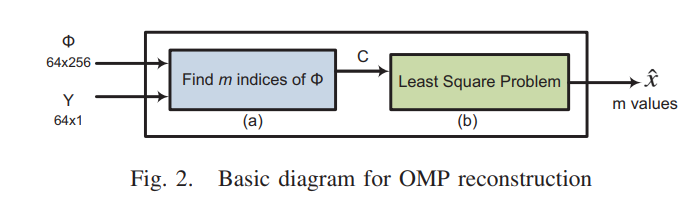
\includegraphics[scale=0.5]{Basic Structure of OMP.png}
        \caption{Basic Structure of OMP}
    \end{center}
\end{figure}

\begin{figure}
    \begin{center}
        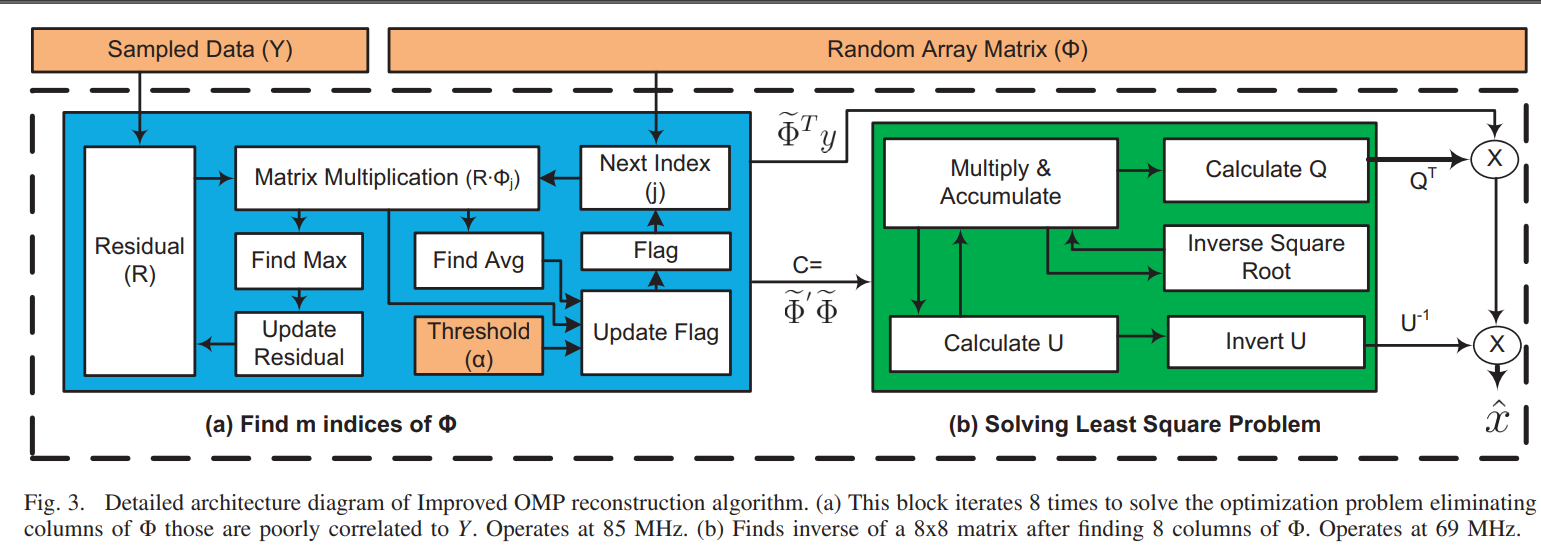
\includegraphics[scale=0.5]{Proposed HArdware Architecture.png}
        \caption{Proposed Hardware Architecture}
    \end{center}
\end{figure}
(c) This paper optimizes the execution of the \textbf{reconstruction technique OMP} which is very widely used in compressed sensing scenario. This paper per se itself doesn't deploy compressed sensing towards any goal but rather seeks to improve what already exists. 
\section{Problem 6}












\end{document}
